\documentclass[a4paper,11pt]{article}

\usepackage[T1]{fontenc}
\usepackage{lmodern}
\usepackage[margin=2.5cm]{geometry}
\usepackage{graphicx}
\usepackage{float}
\usepackage{xcolor}
\usepackage{booktabs}
\usepackage{tabularx}
\usepackage{enumitem}
\usepackage{lastpage}
\usepackage{fancyhdr}
\usepackage{tikz}
\usetikzlibrary{positioning,arrows.meta}
\usepackage[colorlinks=true,urlcolor=orblue,linkcolor=black]{hyperref}

\definecolor{orblue}{HTML}{1F3A93}
\definecolor{ororange}{HTML}{F28C28}
\definecolor{orlight}{HTML}{FFF4E5}
\definecolor{orgrey}{HTML}{5A6670}

\pagestyle{fancy}
\fancyhf{}
\fancyhead[L]{\small\color{orgrey} Office Rush: Technical Overview (work in progress)}
\fancyhead[R]{\small\color{orgrey} G\"orkem \"Ozbek}
\fancyfoot[C]{\small\color{orgrey} \thepage\ / \pageref{LastPage}}
\renewcommand{\headrulewidth}{0.3pt}

\setlength{\parindent}{0pt}
\setlength{\parskip}{0.6em}
\setlist{itemsep=0.15em, topsep=0.3em}
\newcommand{\code}[1]{\texttt{#1}}

\begin{document}

\thispagestyle{empty}
\begin{center}
\vspace*{1.5cm}

\includegraphics[width=6cm]{../screenshots/logo.png}\\[1.2em]
{\Large Run a small company, one busy workday at a time}\\[1.8em]
{\large Technical overview of a mobile game in development}\\[0.4em]
{\color{orgrey} Flutter \textperiodcentered{} Flame \textperiodcentered{} iOS and Android}\\[1.5em]
\fcolorbox{ororange}{orlight}{\parbox{0.8\textwidth}{\centering\bfseries\color{ororange!70!black}
Work in progress: the game is not released yet. Screenshots come from the current development build.}}\\[2em]
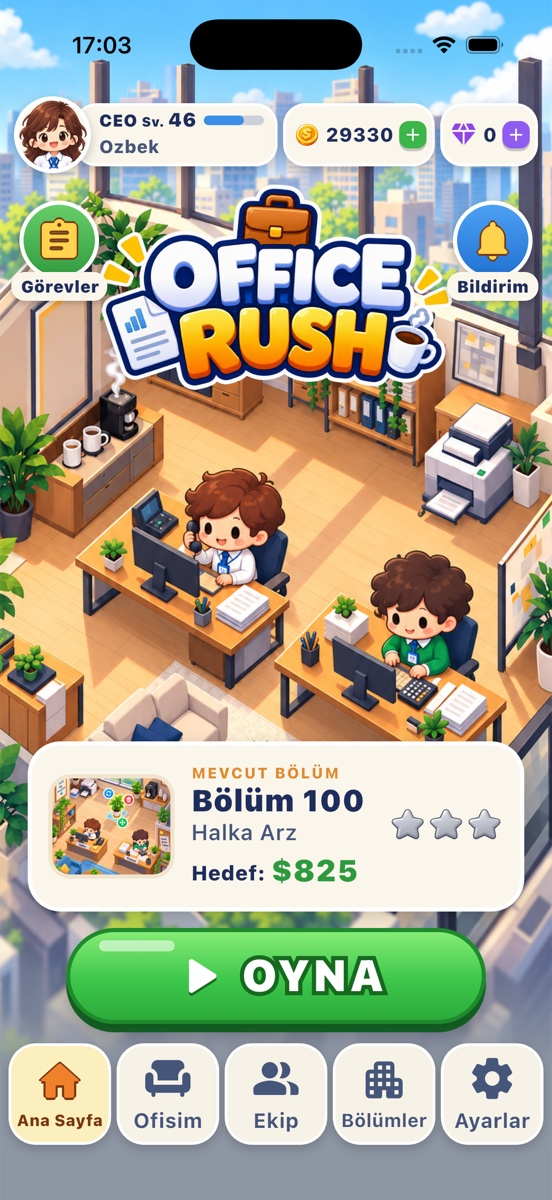
\includegraphics[height=7cm]{../screenshots/01-home.jpg}\hspace{0.3cm}
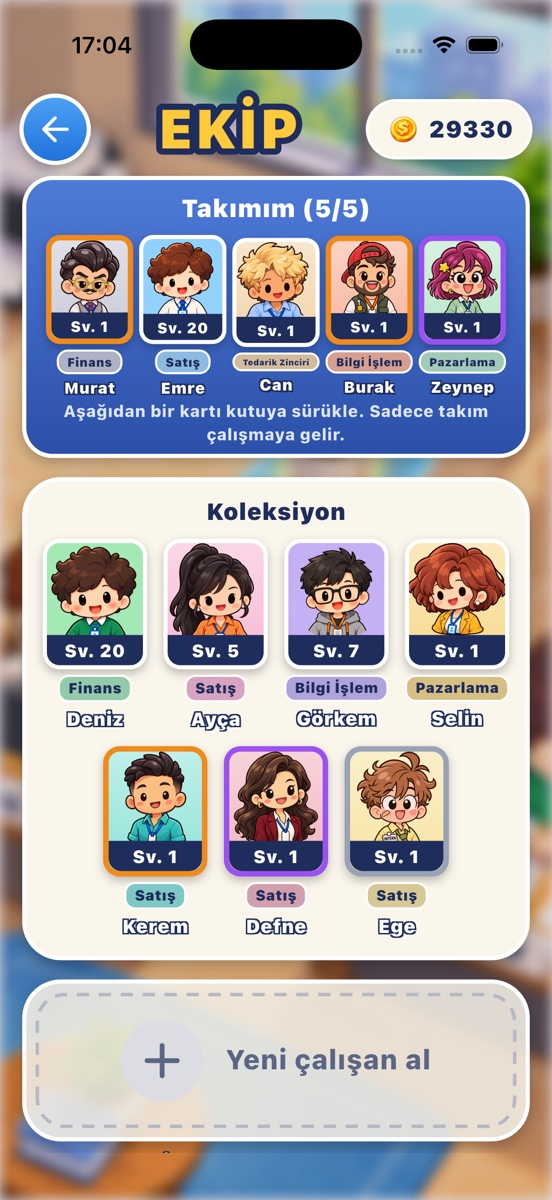
\includegraphics[height=7cm]{../screenshots/03-team.jpg}\hspace{0.3cm}
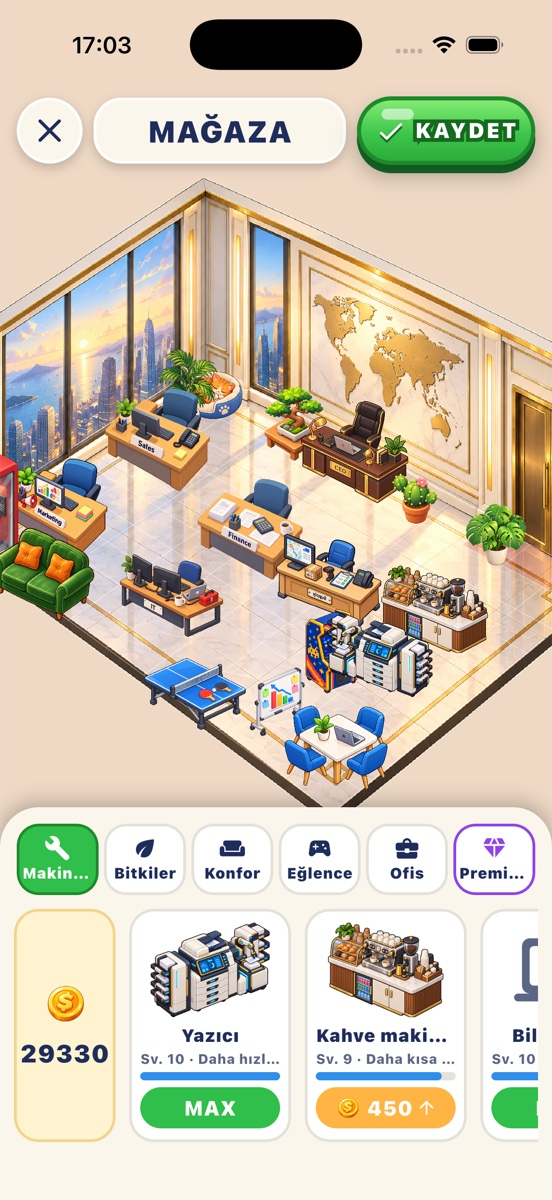
\includegraphics[height=7cm]{../screenshots/04-office-shop.jpg}\\[2.5em]
{\large\bfseries G\"orkem \"Ozbek}\\[0.3em]
{\color{orgrey} November 2026}
\end{center}
\newpage

\tableofcontents
\newpage

\section{Overview}

Office Rush is a casual \textbf{time-management game} for smartphones, set in an office. The player is the CEO of a small company. During a workday of 2 to 3 minutes, they give orders to their employees so that as many customer orders as possible are handled before 6 PM. Between days, the player hires people, improves the team and decorates the office.

The game is designed for short sessions, in portrait mode, and can be played with one hand. It is written with \textbf{Flutter} and the \textbf{Flame} game engine, so one codebase runs on both iOS and Android.

\textbf{Current status.} The game is playable from the first to the last level on the iOS simulator. Art, balancing, sound and some features are still being worked on, and the game has not been published yet.

\section{Gameplay}

\subsection{The order circuit}
Every order goes through the same steps, and each step is a decision of the player:
\begin{enumerate}
  \item The phone rings on a \textbf{Sales} desk. The player taps the employee and chooses \emph{Answer}. Depending on the employee's skill, the call becomes an order or not.
  \item Sales \textbf{prints} the order and brings it to \textbf{Finance}.
  \item Finance \textbf{calculates} the files; the higher the pile on the desk, the slower each calculation.
  \item A \textbf{courier} picks up the finished files. The money only arrives when the courier leaves the office.
\end{enumerate}
Later roles add new steps: \textbf{Supply Chain} manages stock and shipping (and removes the commission of the external distributor), \textbf{IT} repairs breakdowns, and \textbf{Marketing} launches campaigns that bring more calls and VIP customers.

\subsection{Controls and pressure}
\begin{itemize}
  \item Tapping an employee shows large \textbf{contextual action buttons} that change with what the employee can do right now.
  \item Each task has a \textbf{circular timer} (green, orange, red). When it runs out, the customer hangs up and the player loses a reputation star.
  \item Employees have an \textbf{energy bar}; tired employees work slower and need a coffee break.
  \item A long press gives a short \textbf{``Bravo!'' boost} with a cooldown.
\end{itemize}

\subsection{Progression}
\begin{itemize}
  \item \textbf{100 levels in 5 chapters}: small office, one floor, a building, a tower, and an international headquarters. A new mechanic appears every 3 to 5 levels, and each chapter ends with a ``boss day'' (Black Friday, end of quarter, investor visit, product launch, IPO).
  \item \textbf{Team}: a collection of employees with roles and levels. Before each day the player chooses a team of 5 cards.
  \item \textbf{Office editor and shop}: furniture and machines are bought with coins and placed on an isometric grid. Machines can be upgraded (faster printer, shorter coffee break).
  \item \textbf{Economy}: coins, gems, daily missions and in-app purchases.
\end{itemize}

\section{Architecture}

\begin{figure}[H]
\centering
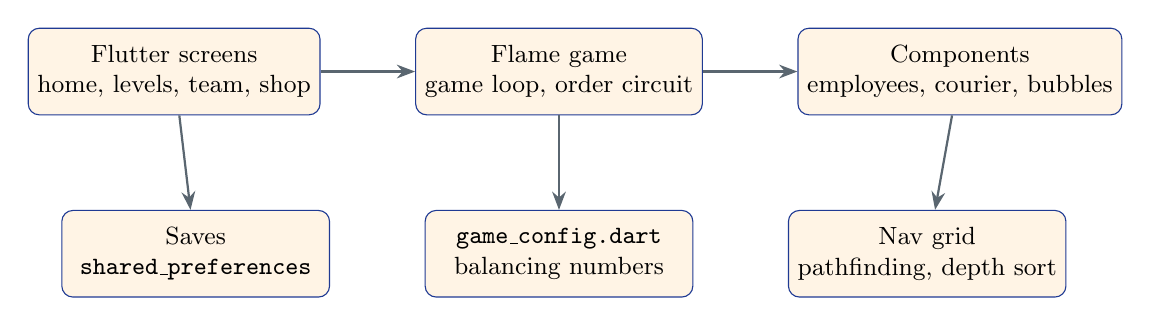
\begin{tikzpicture}[
  box/.style={draw=orblue, fill=orlight, rounded corners, align=center, minimum width=3.4cm, minimum height=1.1cm, font=\small},
  arr/.style={-{Stealth}, thick, orgrey}]
\node[box] (ui) {Flutter screens\\home, levels, team, shop};
\node[box, right=1.2cm of ui] (game) {Flame game\\game loop, order circuit};
\node[box, right=1.2cm of game] (comp) {Components\\employees, courier, bubbles};
\node[box, below=1.2cm of game] (cfg) {\code{game\_config.dart}\\balancing numbers};
\node[box, left=1.2cm of cfg] (save) {Saves\\\code{shared\_preferences}};
\node[box, right=1.2cm of cfg] (nav) {Nav grid\\pathfinding, depth sort};
\draw[arr] (ui) -- (game);
\draw[arr] (game) -- (comp);
\draw[arr] (game) -- (cfg);
\draw[arr] (ui) -- (save);
\draw[arr] (comp) -- (nav);
\end{tikzpicture}
\caption{Main parts of the game}
\end{figure}

\subsection{Main design choices}
\begin{itemize}
  \item \textbf{Levels are data.} A formula computes each level from its number: money target, calls per minute, mix of call types, probability of events, required roles and length of the day, with a little randomness so that two levels never feel the same. Hand-made levels are only used for new roles and boss days.
  \item \textbf{One configuration file.} Every balancing number lives in \code{game\_config.dart}, so the difficulty can be tuned without touching the game code.
  \item \textbf{Isometric scene.} Objects are sorted by their Y position to draw them in the right order, and characters move with pathfinding on an invisible grid, around the furniture placed by the player.
  \item \textbf{Animation in code.} The walking effect (bounce, sway, mirroring) is procedural, so each character only needs a few images.
  \item \textbf{UI in code.} Buttons, panels, timers and badges are drawn in Flutter; images are only used for rooms, furniture, characters and icons. All texts are translated in English, French and Turkish.
\end{itemize}

\section{Tech stack}

\begin{table}[H]
\centering
\begin{tabularx}{\textwidth}{@{}lX@{}}
\toprule
\textbf{Layer} & \textbf{Technologies} \\
\midrule
Game engine & Flutter, Flame \\
Language & Dart (about 19,000 lines) \\
Data & Level formula, configuration file, saves with \code{shared\_preferences} \\
Monetization & \code{in\_app\_purchase}, \code{google\_mobile\_ads} \\
Localization & English, French, Turkish \\
Tests & 17 test files (\code{flutter\_test}, \code{flame\_test}): game logic, pathfinding, order circuit, level formula, office layout \\
\bottomrule
\end{tabularx}
\end{table}

\section{Roadmap}

\begin{table}[H]
\centering
\begin{tabularx}{\textwidth}{@{}lX@{}}
\toprule
\textbf{Date} & \textbf{Milestone} \\
\midrule
September 2026 & Game design document, prototype with simple shapes \\
October 2026 & Order circuit, energy, events, 100-level roadmap, real art \\
November 2026 & Team cards, office editor and shop, daily missions, in-app purchases \\
\textbf{In progress} & Balancing, polish, sounds, more animations \\
Next & Beta on TestFlight and Google Play, then public release \\
\bottomrule
\end{tabularx}
\end{table}

\section{What I am learning}
\begin{itemize}
  \item Structuring a game with an entity-component engine inside a Flutter application.
  \item Data-driven design: generating 100 levels from one formula and one configuration file.
  \item Pathfinding and isometric rendering on a small screen.
  \item Game feel: timers, feedback, difficulty curve and one-hand controls.
  \item Testing game logic automatically.
  \item The rules of free-to-play mobile games: in-app purchases, ads and store policies.
\end{itemize}

\end{document}
